%
% AI Paper by Fahad Uddin
%


\documentclass[12pt]{article}
\usepackage{geometry}
\geometry{letterpaper}
\usepackage{doc}
\usepackage{url}
\usepackage{graphicx}
\usepackage{epstopdf}
\title{Implementing Neural Network with Backpropagation on CIFAR-10 Dataset using C++}

\author{
	%\large
	\mbox{}\\ %
	\\
	\\
	\textsc{Fahad Uddin}
	\qquad
	\mbox{}\\ %
	Department of Computer Science\\
	The City College of New York\\
	New York, New york\\
	\\
	\texttt{fuddin003@citymail.cuny.edu}
	\\
	\\
	\\
	\\
	\\
	\\
	\\
	\\
	\\
	\mbox{}\\ %
	Artificial Inteligence - CS I1500\\
	Fall, 2019\\
	\\
	\normalsize
	\normalsize
}

\date{\today}



\begin{document}

% Add the title section.
\maketitle
\pagenumbering{roman}                   % roman page number for toc
\setcounter{page}{0}                    % make it start with "0"

\pagebreak

% Add an abstract.
\begin{abstract}{
We have seen a rising interest in multi-layer neural networking in recent years on all kinds of industries, from data science to robotics, from big data to the industrial complex. These applications are used for numerous image processing computer vision activities. In this paper, I will discuss how to implement the backpropagation algorithm in a multi-layer neural network. I will be using a popular CIFAR-10 dataset to train the network. CIFAR-10 dataset contains thousands of pictures that we can use to train the network and find anticipated results.
}
\end{abstract}
% Add various lists on new pages.
\pagebreak

\tableofcontents

\pagebreak


\section{Introduction}

The neural network at its highest level is simple, all it does you give it some inputs as binary mode and it will give you a prediction as an output. based on the output you can decide whether to keep continue to get the output till you get the desired result or to stop with the current out. Backpropagation is an algorithm to train the neural network. The backpropagation used in a feed-forward artificial neural network. We can use this algorithm to train large deep learning networks. In this paper, we will discuss how to implement the algorithm in a neural network. It is very important to learn the basic functions and it will help us to implement the mathematics on a real-life data set using a c++ program.\cite{BOOK:1}

\section{Neural Network}

Neural networks are computing systems inspired by the biological neural network. The artificial neural network learns to perform by observing examples without specific rules. Before learning how back-propagation works we need to learn more about neural networks. We need to learn a basic neural network specifically multi-layer perception. A multi-layer neural network is a common kind of neural network. Every layer can have a various amount of neurons. Each neuron would be connected to each neuron of the previous or next layer.


 Figure 1 shows a small example of a multilayer neural network, here every circle is a neuron. This network will take three inputs on its input level, each will be connected to three neurons of the hidden layer. The hidden layer has three neurons, each will also be connected to two output neurons of the output layer.


\begin{figure}
	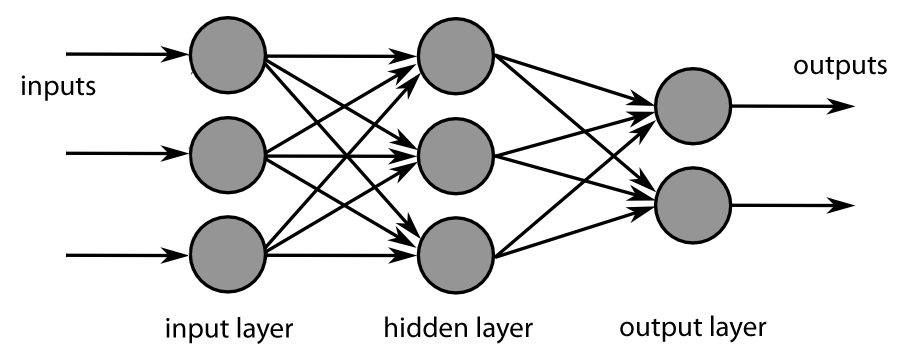
\includegraphics[width=\linewidth]{images/multi-layer.png}
	\caption{Multi-layer Neural Network.}
	\label{fig:multi-layer}
\end{figure}

\subsection{Inputs}
Inputs are the layer where data are being consumed. We can create a number of different channels from which data can be fed. The target of data being fed is to get a prediction from the data. We have to break into binary signals. We can create a different channel for different binary signals. Each channel will represent a neutron.

\subsection{Training Set}
The training set would be the inputs are being fed into the network. In our case it CIFAR-10 dataset. The training set would be used for training the network for a certain scope from which the network can make a prediction.

\subsection{Outputs}
The neural network has an output level. The outputs can be valued between 0 to 1. Also could be Boolean or discrete value.

\subsection{Activation Function}
Every neuron has a numeric weight. The weights and the sigmoid function are used to determine the output for each neuron. In a neural network, our objective is to take weight space to count and determine the output.

\[\sigma (x) =\frac{1}{1 + e^-x}\]
\label{eq:sigmoid}


\subsection{Weight Space}
Every neuron has a numeric weight. The weights and the sigmoid function are used to determine the output for each neuron. In a neural network, our objective is to take weight space to count and determine the output.

\subsection{Initialization}
Initialization refers to the setting of the weights at the beginning of the calculation. We can determine the weights randomly, we can also assign them and start optimizing from the input layer with the bias node. We have to make sure each signal is passing forward with the right calculation.

\subsection{Forward Pass}
The forward pass refers to taking the input into count, using activation function, weights and the bias node we are passing forward the output to the next level. After input level comes to the hidden layer. We have to do the same calculation for the hidden layer. The output for the hidden layer will go to the output layer.

\subsection{Gradient Descent}
The network will be trained using a mathematical technique called gradient descent. By calculating the gradient of a function we can determine the error of the network. We will have the partial derivatives of all weights and biases. We will multiply the gradient by a small learning rate value. Then subtract the derivatives from the weights and biases to decrease the error amount. This is called gradient descent.



\section{Neural Network Learning}
Neural Network learning happens in six stages, at the end of these stages the model would be ready to make a prediction. Base on that we can redefine and restart the process again. 

In order to write the algorithm on a c++ code we need to come out with a plan. A step by step way to implement the algorithm and train the model.

\begin{quote}
1. Initialization\\
2. Forward Propagation\\
3. Error Function\\
4. Back-Propagate Error Function\\
5. Predict\\
6. Iterate Convergence\\
\end{quote}  

\newpage
\begin{figure}
	\centering
	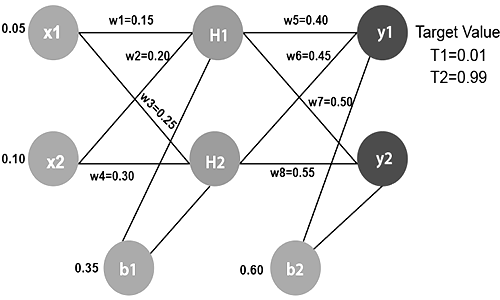
\includegraphics[width=100mm]{images/layers-weight.png}
	\caption{Multi-layer Neural Network with weight.}
	\label{fig:layer-weight}
\end{figure}

\section{Initialization}
We would need a class initiation, where we could define the functions responsible for creating and defining the network architecture, various weight matrices, bias vector.

Every neuron has weight which we should maintain. Every input neuron will have weight and bias node also have weight. We would need to store the weights to use them throughout the program. It is better to assign a small number between 0 to 1 for the weights.

A network architecture have different layers. The input layer is the starting layer for our training data set. After that comes the hidden layer, then the output layer. We can architect layers as arrays and the whole network will be a network of arrays.

In figure 2 the initial values for input x1, x2 and bias nodes b1, b2 are,

\[x1 = 0.05, x2 = 0.10\]
\[b1 = 0.35, b2 = 0.60\]

Initial weights are,

\[w1 = 0.15, w2 = 0.20, w3 = 0.25, w4 = 0.30\]
\[w5 = 0.40, w6 = 0.45, w7 = 0.50, w8 = 0.55\]

Target values are,

\[T1 = 0.01, T2 = 0.99\]

Now our task is to calculate the error function from these initial values.

\section{Forward Propagation}

We can calculate an output from a neural network by propagating an input signal through each layer until the output layer outputs its values. We call this forward-propagation.




To find the value of H1 we first multiply the input value from the weights as

\[H1=x1*w1+x2*w2+b1\]
\[H1=0.05*0.15+0.10*0.20+0.35\]
\[H1=0.3775\]


To calculate the final result of H1, we performed the sigmoid function as

\[H1_{FInal}=\frac{1}{1+\frac{1}{e^{H1}}}\]
\[H1_{FInal}=\frac{1}{1+\frac{1}{e^{0.3775}}}\]
\[H1_{Final}=0.59326992\]


We will calculate the value of H2 in the same way as H1
\[H2=x1*w3+x2*w4+b1\]
\[H2=0.05*0.25+0.10*0.30+0.35\]
\[H2=0.3925\]


To calculate the final result of H2, we performed the sigmoid function as

\[H2_{FInal}=\frac{1}{1+\frac{1}{e^{H2}}}\]
\[H2_{FInal}=\frac{1}{1+\frac{1}{e^{0.3925}}}\]
\[H2_{Final}=0.596884\]


Now, we calculate the values of y1 and y2 in the same way as we calculate the H1 and H2.

To find the value of y1, we first multiply the input value i.e., the outcome of H1 and H2 from the weights as

\[y1=H1*w5+H2*w6+b2\]
\[y1=0.5932699*0.40+0.5968843*0.45+0.60\]
\[y1=1.1059059\]

To calculate the final result of y1 we performed the sigmoid function as

\[y1_{FInal}=\frac{1}{1+\frac{1}{e^{y1}}}\]
\[y1_{FInal}=\frac{1}{1+\frac{1}{e^{1.105905}}}\]
\[y1_{Final}=0.751365\]


We will calculate the value of y2 in the same way as y1

\[y2=H1*w7+H2*w8+b2\]
\[y2=0.5932699*0.50+0.5968843*0.55+0.60\]
\[y2=1.2249214\]

To calculate the final result of H1, we performed the sigmoid function as

\[y2_{FInal}=\frac{1}{1+\frac{1}{e^{y2}}}\]
\[y2_{FInal}=\frac{1}{1+\frac{1}{e^{1.2249214}}}\]
\[y2_{Final}=0.772928465\]

Our target values are 0.01 and 0.99. Our y1 and y2 value is not matched with our target values T1 and T2.

Now, we will find the total error, which is simply the difference between the outputs from the target outputs. The total error is calculated as

\[E_{Total}=\sum\frac{1}{2}(target - output)^{2}\]

\[E_{Total}=\frac{1}{2}(T1 - y1_{Final})^{2}+\frac{1}{2}(T2 - y2_{Final})^{2}\]

\[E_{Total}=\frac{1}{2}(0.01 - 0.751365)^{2}+\frac{1}{2}(0.99 - 0.772928465)^{2}\]

\[E_{Total}=0.274811084+0.0235600257\]

\[E_{Total}=0.29837111\]

Now, we will backpropagate this error to update the weights using a backward pass.

\section{Back-Propagate Error Function}
To update the weight, we calculate the error correspond to each weight with the help of a total error. The error on weight w is calculated by differentiating total error with respect to w.

\[Error_{w}=\frac{\sigma E_{Total}}{\sigma W}\]

We perform backward process so first consider the last weight w5 as

\[Error_{w5}=\frac{\sigma E_{Total}}{\sigma w5}\]


\[E_{Total}=\frac{1}{2}(T1 - y1_{Final})^{2}+\frac{1}{2}(T2 - y2_{Final})^{2}\]


From the second equation, it is clear that we cannot partially differentiate it with respect to w5 because there is no any w5. We split equation one into multiple terms so that we can easily differentiate it with respect to w5 as


\[\frac{\sigma E_{total}}{\sigma w5}=\frac{\sigma E_{total}}{\sigma y1_{final}}*\frac{\sigma y1_{final}}{\sigma y1}*\frac{\sigma y1}{\sigma w5}\]


Now, we calculate each term one by one to differentiate Etotal with respect to w5 as


\[\frac{\sigma E_{total}}{\sigma y1_{final}}=0.74136507\]

\[\frac{\sigma y1}{\sigma w5=0.0.5968843}\]
	
\[Error_{w5}=0.08216704\]

Now, we will calculate the updated weight w5new with the help of the following formula

\[w5_{new}=w5-\eta *\frac{\sigma E_{Total}}{\sigma w5}\]

\[w5_{new}=0.35891648\]

In the same way, we calculate w6new,w7new, and w8new and this will give us the following values

\[w6_{new}=0.48666186\]
\[w7_{new}=0.511301270\]
\[w8_{new}=0.561370121\]


In the same way, we calculate w1new,w2new, w3new, and w4new and this will give us the following values


\[w1_{new}=0.14978071\]
\[w2_{new}=0.19956143\]
\[w3_{new}=0.24975114\]
\[w4_{new}=0.29950229\]

Now we have calculated the new weights.


\section{Train Network}

The network would be trained using gradient decent. Training network involves multiple iteration of exposing dataset to the network and for each line of input we need to do forward propagation for the inputs, backwordpropagate the error and update the network weights.

We need the gradient vector of the cost function, aka the partial derivatives of all the weights and the biases for the cost. Backpropagation gets you the gradient vector, but it isn’t the only way to do so! Another way to do it is to use dual numbers. 

Using dual numbers, you would evaluate the output of the network, using dual numbers instead of floating point numbers, and at the end you’d have your gradient vector. It’s not quite as efficient as backpropagation (or so I’ve heard, I haven’t tried it), but if you know how dual numbers work, it’s super easy to implement.


\section{Predict}

We know how forward propagate works for an input pattern to get an output. This is all we need to do to make a prediction. We can use the output values themselves directly as the probability of a pattern belonging to each output class.

It may be more useful to turn this output back into a crisp class prediction. We can do this by selecting the class value with the larger probability. This is also called the arg max function.

Below is a function named predict() that implements this procedure. It returns the index in the network output that has the largest probability. It assumes that class values have been converted to integers starting at 0.

\section{Iterate Convergence}

The weights would be updated a small delta step at every time, many iteration are rquired in order to get the network to learn. After every iteration the gradient descent will update the weights for less and less global less error function. The amount of iteration are random, it would be defined by the way the network is learning. Th elearning rate the network meta-parameters and the optimization method are used for the less error function

\section{Result}

 Total error 0.298371109 on the network for the forward pass 0.05 and 0.1 inputs. In the first round of Backpropagation, the total error is down to 0.291027924. After repeating this process, the total error is down to 0.0000351085. At this point, the outputs neurons generate 0.159121960 and 0.984065734 i.e., nearby our target value when we feed forward the 0.05 and 0.1.

\section{CIFAR-10 Dataset}
 The CIFAR-10 datset is the subset of 80 million small images. This dataset were collected by Alex Krizhevsky, Vinod Nair, and Geoffrey Hinton.
 
The CIFAR-10 dataset have 60,000 32*32 colour images in 10 classes. 6000 images per class. There are 50000 training images and 10,000 test images. 
This dataset contains images of airplane, automobile, bird, cat, deer, dog, frog, horse, ship and truck

The classes are mutually exclusive. We are going to use this dataset to train our network and make a prediction.


\section{Conclusion}


I have learned a great deal about neural network while reaserching for this paper. My research on various site helped me grasp the basics of backpropagation and neural network model training. There alot of scope to work on. We can try larger or smaller networks trained for longer or shorter. See if we can get better performance on the dataset.\cite{ARTICLE:1}

We can experiment with different weight initialization techniques. we can also add support for more hidden layers, trained in just the same way as the one hidden layer used in this tutorial.

\bibliography{ai-papers}
\bibliographystyle{ieeetr}

\end{document}
